\clearpage
\section{Additional results}\label{app:more}
\Cref{tab:side} compares DistilBERT's truncated hash encodings with shorter hashes that fit its input limit
(\cref{sec:method}). \Cref{fig:exp2} shows the within-dataset macro-F1 of \cref{tab:exp2} as a chart, and
\cref{tab:accuracy} gives the within-dataset test accuracy, for comparison with the SecurityBERT paper. For the
cross-dataset runs of Experiment 3, \cref{fig:exp3} shows every train/test pair and \cref{fig:offdiag} summarises
the off-diagonal scores per method.

\begin{table}[H]
  \centering
  \caption{Appendix B. DistilBERT side runs: shorter hashes (nothing truncated) vs.\ the main runs, which are truncated to the
    model's input limit.}
  \label{tab:side}
  \gentable{exp2_side_runs}
\end{table}

\begin{figure}[H]
  \centering
  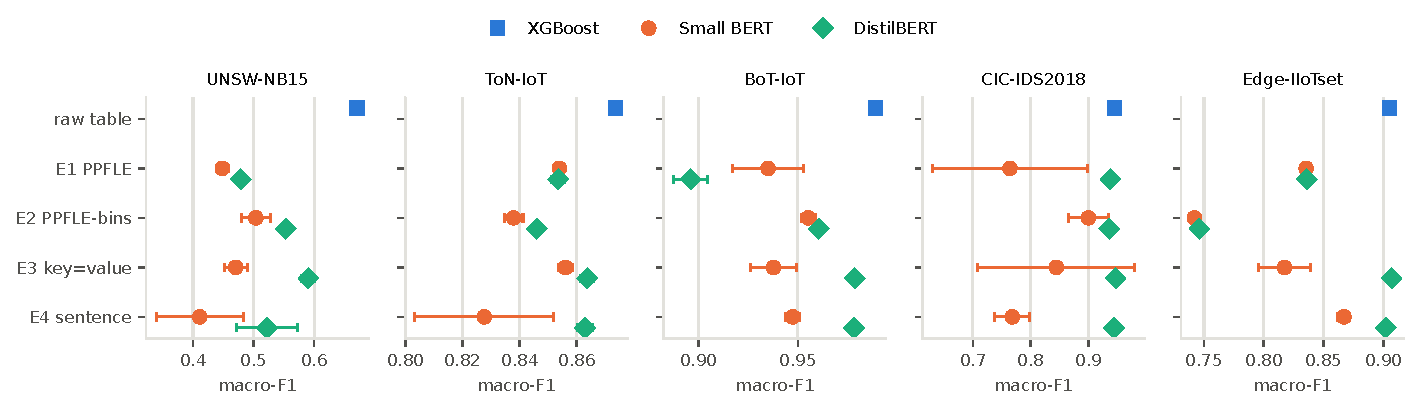
\includegraphics[width=\linewidth]{exp2_within_macro_f1}
  \caption{Appendix B. Within-dataset macro-F1 per encoding and model (bars: std over seeds). Each panel has
    its own x-range.}
  \label{fig:exp2}
\end{figure}

\begin{table}[H]
  \centering
  \caption{Appendix B. Test accuracy (multiclass), for comparison with the SecurityBERT paper.}
  \label{tab:accuracy}
  \gentable{exp2_within_accuracy}
\end{table}

\begin{figure}[H]
  \centering
  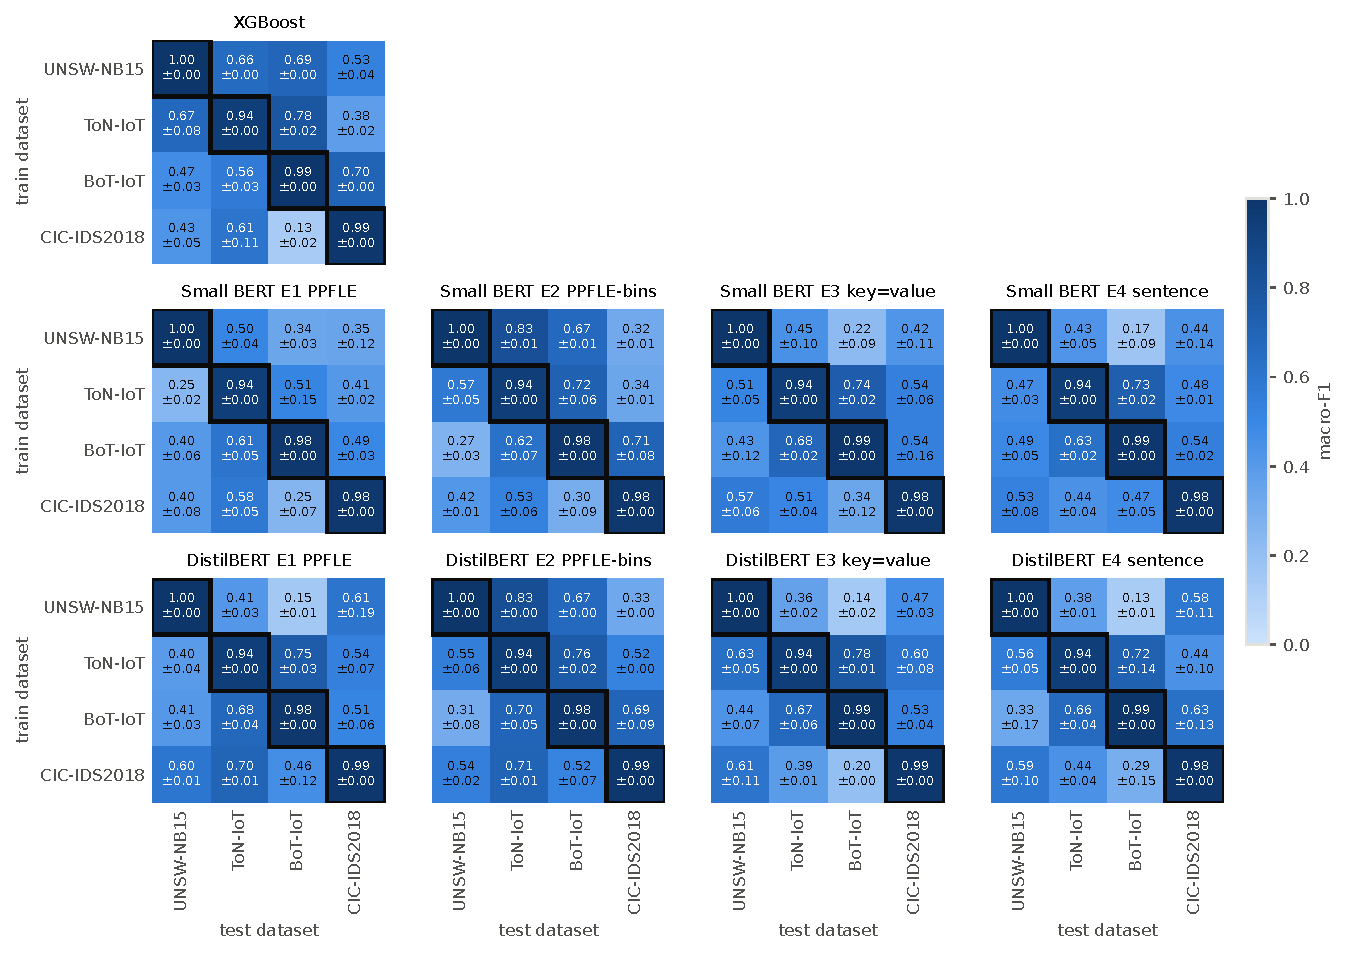
\includegraphics[width=\linewidth]{exp3_heatmaps_grid}
  \caption{Appendix B. Binary macro-F1, trained on the row dataset and tested on the column dataset (diagonal outlined).}
  \label{fig:exp3}
\end{figure}

\begin{figure}[H]
  \centering
  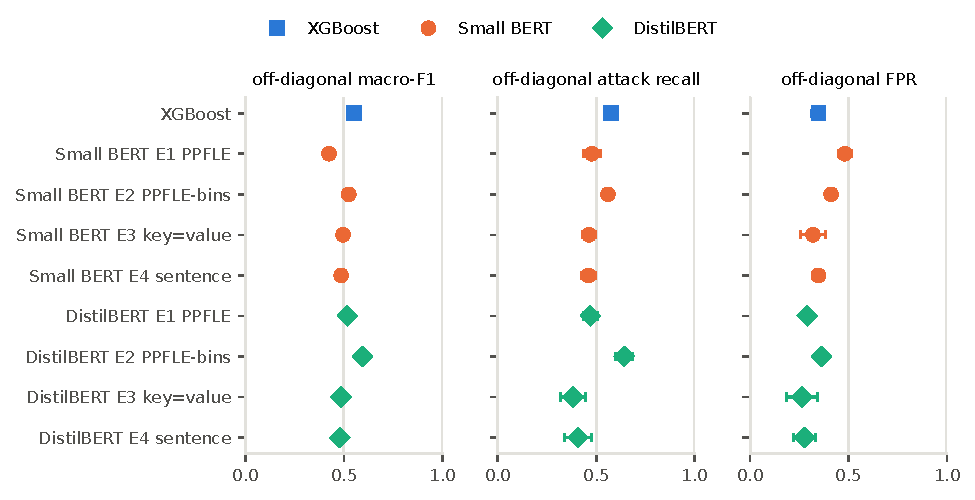
\includegraphics[width=0.85\linewidth]{exp3_offdiag}
  \caption{Appendix B. Off-diagonal macro-F1, attack recall and FPR per method.}
  \label{fig:offdiag}
\end{figure}
